\documentclass{article}

\usepackage[utf8]{inputenc}
\usepackage[T1]{fontenc}
\usepackage{lmodern}
\usepackage{amsmath}
\usepackage{amsfonts}
\usepackage{amssymb}
\usepackage{booktabs}
\usepackage{graphicx}
\usepackage{hyperref}

\title{Five-Step Gated Quintic Newton--Schulz}
\author{}
\date{}

\begin{document}
\maketitle

\begin{abstract}
This note describes the exact gated five-step Newton--Schulz variant used for
GatedMuon. The transform keeps the tuned five-step quintic polar approximation,
but multiplies the result by a smooth gate with fixed threshold
\(\tau=10^{-5}\). The gate prevents very small singular values from being
amplified into full-strength Muon update directions.
\end{abstract}

\section{Setup}

Let \(M \in \mathbb{R}^{m\times n}\) be the momentum or Nesterov momentum
matrix. Orient it so that the smaller dimension is on the left, and normalize
by its Frobenius norm:
\[
    X = \frac{M}{\|M\|_F+\varepsilon}.
\]
If
\[
    X = U \operatorname{diag}(\sigma_i) V^\top,
\]
then ordinary Muon aims to output the polar factor
\[
    U V^\top,
\]
which maps every nonzero singular value to \(1\).

The gated five-step variant instead outputs approximately
\[
    U \operatorname{diag}\!\left(g_\tau(\sigma_i)\right) V^\top,
    \qquad
    \tau = 10^{-5},
\]
where
\[
    g_\tau(\sigma)
    =
    \frac{\sigma^2}{\sigma^2+\tau^2}.
\]
Thus singular values much larger than \(10^{-5}\) behave almost like Muon,
while singular values below \(10^{-5}\) are suppressed.

\section{Five Quintic Steps}

Starting from \(Y_0=X\), apply exactly five tuned quintic Newton--Schulz steps:
\[
    Y_{j+1}
    =
    a_jY_j
    +
    b_j(Y_jY_j^\top)Y_j
    +
    c_j(Y_jY_j^\top)^2Y_j,
    \qquad
    j=0,\ldots,4.
\]
The coefficient rows \((a_j,b_j,c_j)\) are
\[
\begin{array}{ccc}
4.0848 & -6.8946 & 2.9270\\
3.9505 & -6.3029 & 2.6377\\
3.7418 & -5.5913 & 2.3037\\
2.8769 & -3.1427 & 1.2046\\
2.8366 & -3.0525 & 1.2012
\end{array}
\]
These five steps approximate \(UV^\top\). For tiny singular values, the
linear part dominates, so the ungated small-value amplification is roughly
\[
    \prod_{j=0}^4 a_j \approx 493.
\]
For example, before gating,
\[
    10^{-5} \mapsto 4.9\times 10^{-3},
    \qquad
    2\times 10^{-4} \mapsto 9.8\times 10^{-2}.
\]

\section{The \texorpdfstring{\(\tau=10^{-5}\)}{tau=1e-5} Gate}

After the five quintic steps, apply the gate using the singular values of the
original normalized matrix \(X\), not the singular values after the iteration:
\[
    D
    =
    U
    \operatorname{diag}\!\left(
        \frac{\sigma_i^2}{\sigma_i^2 + 10^{-10}}
    \right)
    V^\top
    \quad
    \text{approximately}.
\]
Equivalently,
\[
    D \approx G_\tau Y_5,
\]
where
\[
    X X^\top
    =
    U \operatorname{diag}(\sigma_i^2) U^\top
\]
and
\[
    G_\tau
    =
    U
    \operatorname{diag}
    \left(
        \frac{\sigma_i^2}{\sigma_i^2+10^{-10}}
    \right)
    U^\top.
\]
This uses only the small Gram matrix \(XX^\top\).

At the threshold,
\[
    g_{10^{-5}}(10^{-5}) = \frac{1}{2}.
\]
Above the threshold the gate is nearly one:
\[
    g_{10^{-5}}(10^{-4})
    =
    \frac{10^{-8}}{10^{-8}+10^{-10}}
    \approx 0.99.
\]
Below the threshold it decays quadratically:
\[
    g_{10^{-5}}(10^{-6})
    =
    \frac{10^{-12}}{10^{-12}+10^{-10}}
    \approx 0.0099.
\]

\begin{figure}[t]
    \centering
    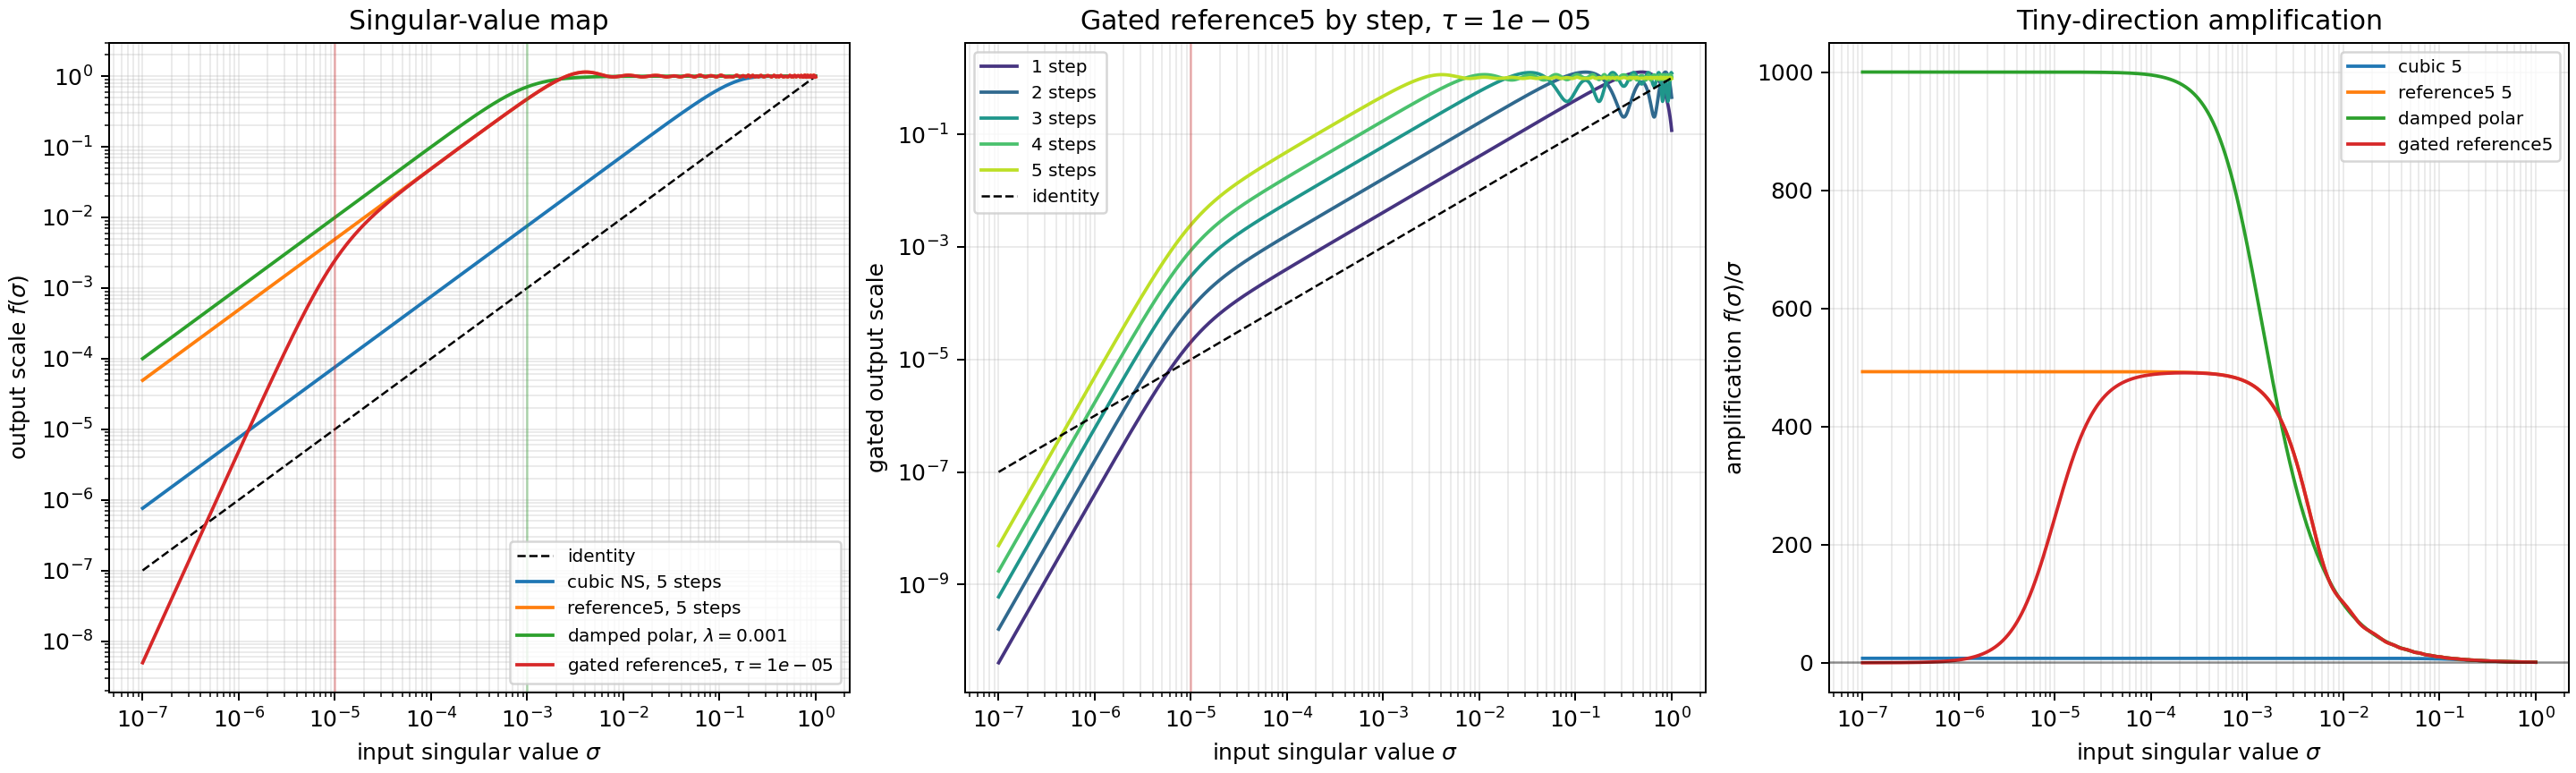
\includegraphics[width=\linewidth]{results/gated_muon_reference5_tau_1e-5.png}
    \caption{Scalar singular-value response for the five-step tuned quintic
    Newton--Schulz transform with gate threshold \(\tau=10^{-5}\). The middle
    panel shows the gated response after each of the five steps.}
    \label{fig:gated-five-step-response}
\end{figure}

\section{Shape Scaling}

The gated transform is still used with Muon's shape-aware learning-rate
prefactor
\[
    \sqrt{\frac{\mathrm{fan\_out}}{\mathrm{fan\_in}}}.
\]
The reason is the same as in the Muon derivation. For a linear layer
\[
    y = Wx,
\]
the RMS-to-RMS operator norm satisfies
\[
    \|D\|_{\mathrm{RMS}\to\mathrm{RMS}}
    =
    \sqrt{\frac{\mathrm{fan\_in}}{\mathrm{fan\_out}}}\,
    \|D\|_2.
\]
Plain Muon chooses an update with \(\|D\|_2\approx 1\), so multiplying by
\[
    \sqrt{\frac{\mathrm{fan\_out}}{\mathrm{fan\_in}}}
\]
makes the RMS-to-RMS size of the update approximately independent of the
matrix shape.

The gate only reduces singular values:
\[
    0 \le g_{10^{-5}}(\sigma) \le 1.
\]
Therefore the gated update has spectral norm at most the Muon polar update:
\[
    \|D^{\mathrm{gated}}\|_2 \le 1.
\]
Keeping the same shape scaling preserves the Muon interpretation of the
learning rate as controlling RMS output perturbation, while the gate can make
the update smaller when the relevant singular directions are near the
\(10^{-5}\) threshold.

\end{document}
